\section{Experiments}
\label{sec:experiments}

We evaluate PivotRL with three questions. First, when trained on the same prompts and expert trajectories as supervised fine-tuning (SFT), does PivotRL achieve larger in-domain gains while better preserving out-of-domain (OOD) capability? Second, on SWE-Bench, where end-to-end reinforcement learning (E2E RL) is a natural baseline, can pivotRL attain competitive accuracy with substantially lower rollout burden? Third, do the two components of PivotRL---informative pivot selection and functional reward---each matter in isolation?

Unless otherwise stated, all experiments use \texttt{Qwen3-30B-A3B-Thinking-2507} as the base model, Nemo-RL \citep{nemo-rl} as the training framework, and Nemo-Gym \citep{nemo-gym} for environment rollouts. For all SFT--PivotRL comparisons, we use the same prompts and expert trajectories; the only difference is the training objective. Each single-domain experiment produces a separate post-trained policy. For a model trained on one target domain, we define OOD change as the score difference relative to the base model on held-out benchmarks outside that training domain.

\subsection{Experimental questions and benchmarks}
\label{sec:exp_questions_benchmarks}

We evaluate PivotRL on four agentic benchmarks spanning the domains studied in this paper.

\begin{itemize}
  \item \textbf{$\tau^2$-Bench} \citep{barres2025tau2bench} evaluates conversational tool use in multi-turn customer-service environments. It contains three subsets: Retail and Airline \citep{yao2024taubench}, which primarily test agent tool use, and Telecom, which additionally includes user tool calls. We keep the user simulator fixed to \texttt{Qwen3-235B-A22B-Instruct-2507} in all evaluations.
  
  \item \textbf{SWE-Bench Verified} \citep{jimenez2024swebench} evaluates software-engineering agents on real GitHub issues that require understanding the problem, localizing the bug, and producing a correct patch. We use the verified subset of 500 tasks and evaluate with the OpenHands harness.

  \item \textbf{Terminal-Bench} \citep{tbench_2025} evaluates bash-terminal agents on tasks ranging from filesystem navigation and coding to system administration and more complex problem-solving. We evaluate on TBCore-v1.1 with the Terminus-2 harness.

  \item \textbf{BrowseComp} \citep{wei2025browsecompsimplechallengingbenchmark} evaluates web-search agents on difficult information-seeking questions that often require long trajectories with many search calls and nontrivial evidence synthesis.
\end{itemize}

Across these domains, an action always denotes the full assistant completion at a model-call boundary. Depending on the benchmark, this may be a conversational tool-use step, a tool call in a coding agent trace, a bash command, or a search-related action.

\subsection{Same-data comparison to SFT}
\label{sec:same_data_sft}

We begin with the cleanest comparison in the paper: SFT versus PivotRL under identical training data. This directly tests whether replacing SFT's behavior cloning with PivotRL's on-policy verifier-based RL improves adaptation while reducing catastrophic forgetting.

\begin{table}[t]
\centering
\small
\begin{tabular}{lccccc}
\toprule
\textbf{Benchmark} & \textbf{Base} & \textbf{SFT} & \textbf{PivotRL} & \textbf{$\Delta$ vs Base} & \textbf{$\Delta$ vs SFT} \\
\midrule
$\tau^2$-Bench   & 44.35 & 58.44 & 63.81 & +19.46 & +5.37 \\
SWE-Verified     & 19.07 & 37.40 & 32.67 & +13.60 & -4.73 \\
Terminal-Bench   & 5.42  & 13.75 & 20.00 & +14.58 & +6.25 \\
BrowseComp       & 2.50  & 1.50  & 11.30 & +8.80  & +9.80 \\
\bottomrule
\end{tabular}
\caption{
Single-domain in-domain results.
SFT and PivotRL use the same prompts and expert trajectories.
}
\label{tab:single_domain_main_results}
\end{table}

Table~\ref{tab:single_domain_main_results} shows that PivotRL substantially improves over the base model in all four target domains, reaching 63.81 on $\tau^2$-Bench, 32.67 on SWE-Verified, 20.00 on Terminal-Bench, and 11.30 on BrowseComp. Averaged over the four single-domain settings, PivotRL yields a larger peak in-domain gain than same-data SFT (+14.11 vs. +9.94).

We next evaluate OOD retention. If PivotRL behaves more like on-policy RL than behavior cloning, it should preserve non-target capabilities more effectively than same-data SFT.

\begin{table*}[t]
\centering
\small
\resizebox{\textwidth}{!}{%
\begin{tabular}{l c cc cc cc cc}
\toprule
\multirow{3}{*}{\textbf{Benchmark}} 
& \multirow{3}{*}{\textbf{Baseline}} 
& \multicolumn{8}{c}{\textbf{Training Domain (score + $\Delta$)}} \\
\cmidrule(lr){3-10}
& 
& \multicolumn{2}{c}{$\tau^2$} 
& \multicolumn{2}{c}{SWE} 
& \multicolumn{2}{c}{Terminal} 
& \multicolumn{2}{c}{BrowseComp} \\
\cmidrule(lr){3-4} \cmidrule(lr){5-6} \cmidrule(lr){7-8} \cmidrule(lr){9-10}
& Qwen3-30B 
& sft & rl 
& sft & rl 
& sft & rl 
& sft & rl \\
\midrule
\midrule

\textbf{Peak In-Domain} 
& -- 
& 58.44 (+14.09) & 63.81 (+19.46)
& 37.40 (+18.33) & 32.67 (+13.60)
& 13.75 (+8.33)  & 20.00 (+14.58)
& 1.50 (-1.00)   & 11.30 (+8.80) \\
\midrule

IFBench 
& 52.04 
& 44.42 (-7.62) & 53.29 (+1.25)
& 38.80 (-13.24) & 54.79 (+2.75)
& 24.77 (-27.27) & 49.47 (-2.57)
& 54.35 (+2.31)  & 53.89 (+1.85) \\

AIME25 
& 86.04 
& 76.25 (-9.79) & 85.63 (-0.41)
& 82.29 (-3.75)  & 85.00 (-1.04)
& 21.56 (-64.48) & 82.92 (-3.12)
& 85.21 (-0.83)  & 85.83 (-0.21) \\

MATH500 
& 98.05 
& 98.00 (-0.05) & 98.35 (+0.30)
& 98.30 (+0.25)  & 98.65 (+0.60)
& 63.55 (-34.50) & 98.00 (-0.05)
& 98.30 (+0.25)  & 98.40 (+0.35) \\

LiveCodeBench 
& 66.52 
& 64.98 (-1.54) & 66.96 (+0.44)
& 57.27 (-9.25)  & 66.96 (+0.44)
& 45.15 (-21.37) & 64.54 (-1.98)
& 67.62 (+1.10)  & 66.96 (+0.44) \\

Scicode 
& 36.83 
& 31.95 (-4.88) & 38.68 (+1.85)
& 24.85 (-11.98) & 39.87 (+3.04)
& 9.39 (-27.44)  & 39.13 (+2.30)
& 35.58 (-1.25)  & 37.28 (+0.45) \\

MMLU-Pro 
& 80.84 
& 79.81 (-1.03) & 81.31 (+0.47)
& 78.90 (-1.94)  & 81.13 (+0.29)
& 71.57 (-9.27)  & 80.85 (+0.01)
& 81.13 (+0.29)  & 81.31 (+0.47) \\

MMLU-ProX 
& 78.58 
& 74.31 (-4.27) & 78.92 (+0.34)
& 75.58 (-3.00)  & 78.81 (+0.23)
& 59.13 (-19.45) & 78.49 (-0.09)
& 76.68 (-1.90)  & 78.60 (+0.02) \\

WMT24++ 
& 36.97 
& 34.25 (-2.72) & 36.54 (-0.43)
& 35.69 (-1.28)  & 36.66 (-0.31)
& 6.31 (-30.66)  & 36.48 (-0.49)
& 33.18 (-3.79)  & 36.26 (-0.71) \\

\bottomrule
\end{tabular}%
}
\caption{
Out-of-domain regression across four single-domain training runs.
Each cell shows score followed by per-task $\Delta$ relative to the Qwen3-30B baseline.
All RL--SFT comparisons use identical seed prompts and trajectories.
}
\label{tab:single_domain_ood_full}
\end{table*}

\begin{table}[t]
\centering
\small
\begin{tabular}{l c cc}
\toprule
\textbf{Evaluation} & \textbf{Baseline} & \textbf{Avg $\Delta$ SFT} & \textbf{Avg $\Delta$ RL} \\
\midrule
\textbf{In-Domain (Peak)} & -- & +9.94 & +14.11 \\
\midrule
IFBench        & 52.04 & -10.45 & +0.82 \\
AIME25         & 86.04 & -19.71 & -1.20 \\
MATH500        & 98.05 & -8.58  & +0.30 \\
LiveCodeBench  & 66.52 & -8.41  & -0.16 \\
Scicode        & 36.83 & -8.89  & +1.91 \\
MMLU-Pro       & 80.84 & -3.05  & +0.31 \\
MMLU-ProX      & 78.58 & -7.15  & +0.13 \\
WMT24++        & 36.97 & -9.59  & -0.49 \\
\midrule
\textbf{Avg OOD (All Benchmarks)} & 66.98 & -9.48 & +0.20 \\
\bottomrule
\end{tabular}
\caption{
Average performance change ($\Delta$) relative to the Qwen3-30B baseline across four single-domain training runs.
PivotRL achieves larger average in-domain gains while maintaining near-zero average OOD change, whereas same-data SFT exhibits substantial forgetting.
}
\label{tab:single_domain_ood_avg}
\end{table}

Tables~\ref{tab:single_domain_ood_full} and~\ref{tab:single_domain_ood_avg} show a clear difference between the two objectives. SFT often improves the target domain but at the cost of substantial degradation elsewhere, with an average OOD change of $-9.48$. By contrast, PivotRL preserves general capability much better, with an average OOD change of only +0.20. The strongest failure case for SFT occurs in terminal training, where SFT causes broad OOD collapse while PivotRL remains close to the base model on held-out benchmarks.

\subsection{Comparison to end-to-end RL on SWE-Bench}
\label{sec:swe_e2e}

SWE-Bench is the domain in our suite for which end-to-end RL is the most natural baseline. In this setting, the main question is whether local verifier-based RL can recover a large fraction of E2E RL's benefit while requiring substantially less online interaction.

\begin{table}[t]
\centering
\small
\begin{tabular}{lccc}
\toprule
\textbf{Method} & \textbf{Score} & \textbf{Online Interaction} & \textbf{Training Regime} \\
\midrule
Base model & 19.07 & -- & none \\
Same-data SFT & 37.40 & offline only & behavior cloning \\
PivotRL & 32.67 & [PLACEHOLDER] & local turn-level RL \\
E2E RL & [PLACEHOLDER] & [PLACEHOLDER] & full-trajectory RL \\
PivotRL $\rightarrow$ E2E RL & [PLACEHOLDER] & [PLACEHOLDER] & local RL then full-trajectory RL \\
\bottomrule
\end{tabular}
\caption{
SWE-Bench comparison to end-to-end RL.
The table reports both final accuracy and online interaction cost.
}
\label{tab:swe_e2e}
\end{table}

Table~\ref{tab:swe_e2e} compares PivotRL against full-trajectory RL on SWE-Bench. PivotRL operates with local one-turn or partial rollouts at selected pivots, whereas E2E RL requires repeated full-horizon environment interaction. This experiment isolates the computational tradeoff central to the paper.

\subsection{Component ablations}
\label{sec:component_ablations}

This subsection isolates the two components introduced in Sections~\ref{sec:prelim} and~\ref{sec:pivotrl}: informative pivot selection and functional reward.

\subsubsection{Pivot selection on $\tau^2$-Bench}
\label{sec:tau_pivot_ablation}

We use $\tau^2$-Bench as the main pivot-selection testbed because it is the lowest-cost environment in our suite and therefore supports controlled ablations at scale. Table~\ref{tab:tau_pivot_selection} compares three pivot datasets: random pivots, mixed-outcome pivots, and a stricter difficult mixed-outcome subset. The random-pivot baseline corresponds to the naive local-RL construction from Section~\ref{sec:prelim}.

\begin{table*}[t]
\small
\centering
\setlength{\tabcolsep}{6pt}
\newcolumntype{F}{>{\centering\arraybackslash}p{0.8cm}}
\newcolumntype{C}{>{\centering\arraybackslash}p{0.8cm}}
\begin{tabular}{l|F|F|C|C}
\toprule
& \multicolumn{1}{c|}{\textbf{$\tau^2$-Airline}}
& \multicolumn{1}{c|}{\textbf{$\tau^2$-Retail}}
& \multicolumn{1}{c|}{\textbf{$\tau^2$-Telecom}}
& \multicolumn{1}{c}{\textbf{$\tau^2$-Average}} \\
\midrule
gpt-oss-120b-high
& 55.33 & 58.19 & 67.20 & 60.24 \\
gpt-oss-20b-high
& 43.33 & 50.20 & 52.63 & 48.72 \\
Qwen3-235B-A22B-Thinking-2507
& 50.00 & 66.08 & 46.78 & 54.29 \\
\midrule
Qwen3-30B-A3B-Thinking-2507
& 50.00 & 54.39 & 28.65 & 44.35 \\
\hdashline
Qwen + SFT
& 51.33 & 58.19 & 65.79 & 58.44 \\
Qwen + Random Pivots
& 58.00 & 63.74 & 57.31 & 59.68 \\
Qwen + Mixed-Outcome Pivots
& 61.33 & 66.08 & 56.73 & 61.38 \\
Qwen + Difficult Mixed-Outcome Pivots
& 58.67 & 69.01 & 63.74 & 63.81 \\
\bottomrule
\end{tabular}
\caption{
Effect of pivot selection on $\tau^2$-Bench.
Best checkpoint over training.
Random pivots improve over the base model, mixed-outcome pivots improve further, and difficult mixed-outcome pivots perform best.
}
\label{tab:tau_pivot_selection}
\end{table*}

Table~\ref{tab:tau_pivot_selection} supports the pivot-selection component of the method. Random pivots improve the base model from 44.35 to 59.68 and slightly exceed same-data SFT at 58.44, but they remain below more selective pivot sets. Filtering to mixed-outcome pivots raises accuracy to 61.38, and restricting further to difficult mixed-outcome pivots yields the best result, 63.81.

\begin{figure}[t]
    \centering
    \begin{minipage}{0.48\textwidth}
        \centering
        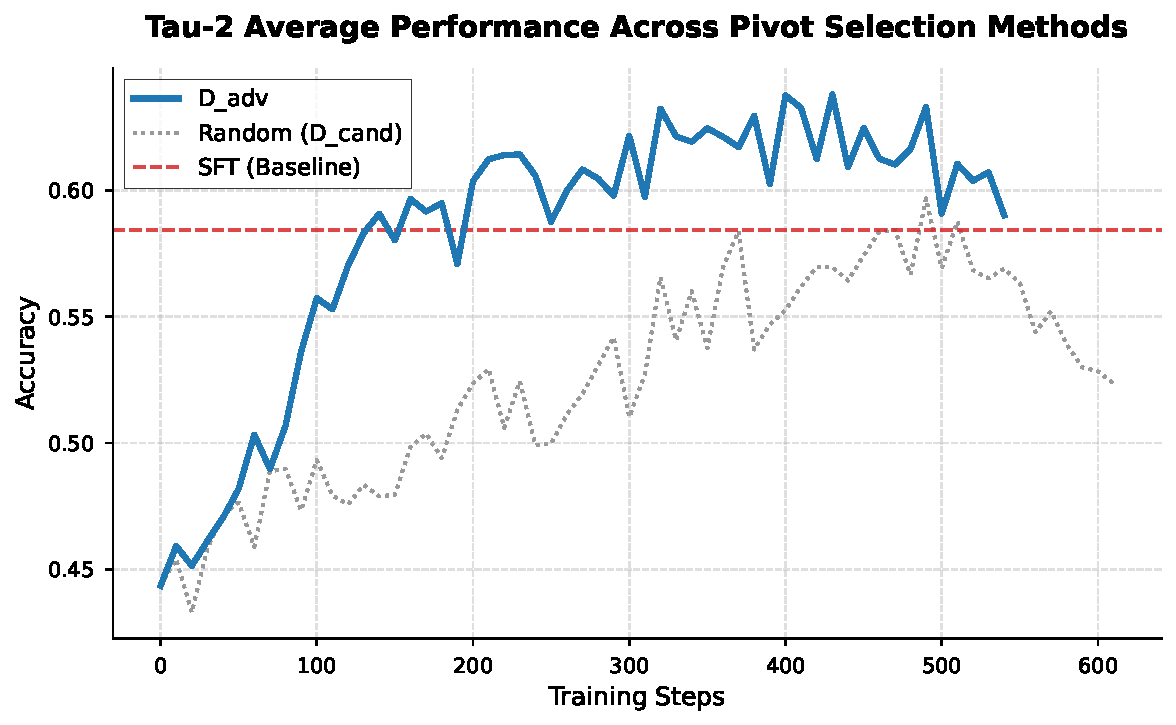
\includegraphics[width=\linewidth]{figures/main_average_validation.pdf}
        \caption{$\tau^2$-Bench accuracy over RL training. Difficult mixed-outcome pivots yield the strongest optimization and outperform same-data SFT.}
        \label{fig:tau_pivot_selection_acc}
    \end{minipage}
    \hfill
    \begin{minipage}{0.48\textwidth}
        \centering
        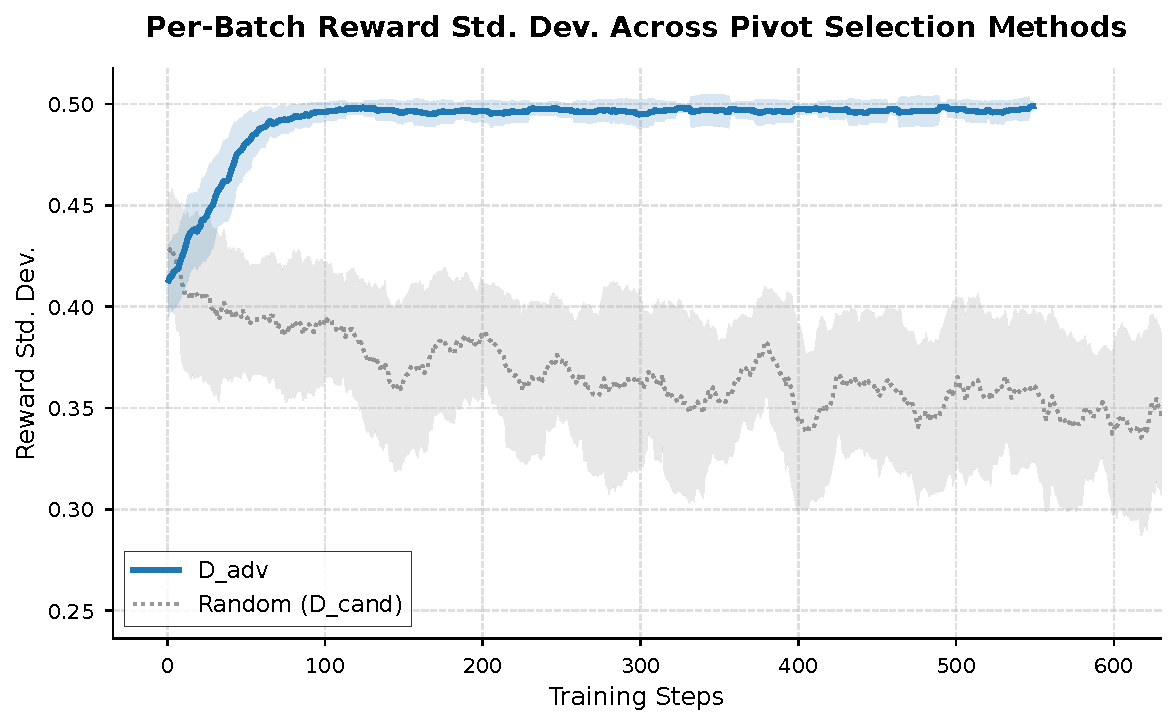
\includegraphics[width=\linewidth]{figures/tau_reward_stddev.pdf}
        \caption{$\tau^2$-Bench training reward standard deviation. More selective pivot datasets maintain higher reward variance during training.}
        \label{fig:tau_reward_std}
    \end{minipage}
\end{figure}

\begin{figure*}[t]
    \centering
    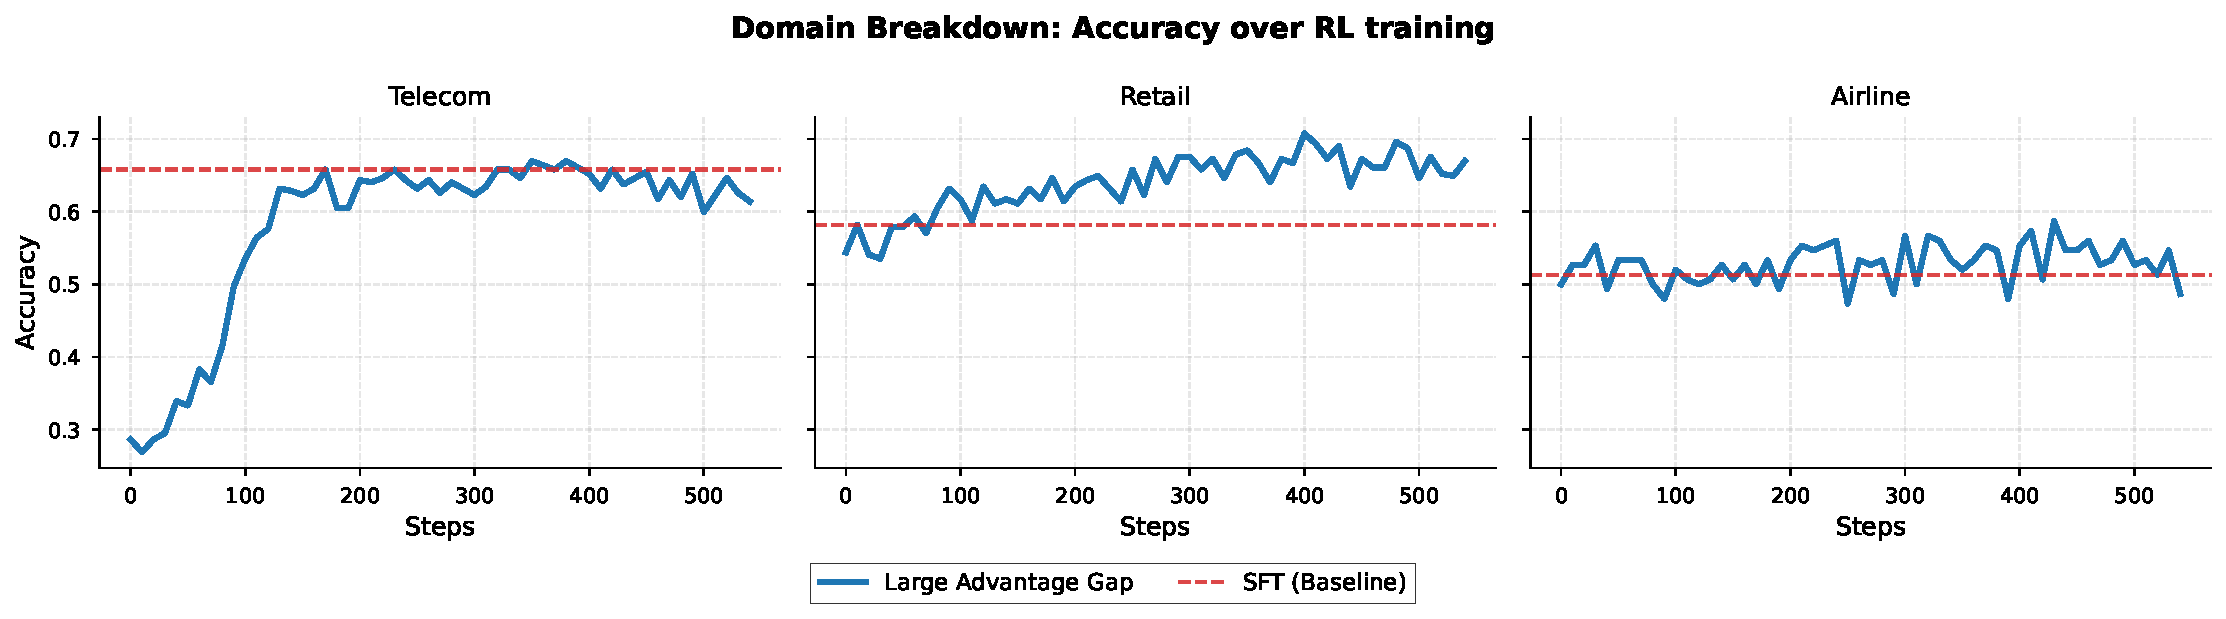
\includegraphics[width=1.0\textwidth]{figures/main_per_domain_validation_difficulty.pdf}
    \caption{Per-domain $\tau^2$-Bench accuracy over RL training for the difficult mixed-outcome pivot set. From left to right: Telecom, Retail, Airline.}
    \label{fig:tau_domain_breakdown}
\end{figure*}

Figures~\ref{fig:tau_pivot_selection_acc} and~\ref{fig:tau_reward_std} show the corresponding optimization behavior. Random pivot sampling quickly collapses to lower per-batch reward variance, indicating that many sampled states provide little or no advantage signal. The mixed-outcome and difficult mixed-outcome pivot sets preserve higher reward variance deeper into training, consistent with Proposition~\ref{prop:mixed}. Figure~\ref{fig:tau_domain_breakdown} shows the per-domain improvement for the strongest pivot set.

\subsubsection{Functional reward and joint 2$\times$2 ablation}
\label{sec:joint_ablation}

We next ablate the two components jointly by crossing pivot selection with reward design:
\[
\{\text{random pivots},\ \text{informative pivots}\}
\quad \times \quad
\{\text{strict reward},\ \text{functional reward}\}.
\]
In this ablation, the naive baseline corresponds to \emph{random pivots + strict reward}, while full PivotRL corresponds to \emph{informative pivots + functional reward}.

\begin{table}[t]
\centering
\small
\begin{tabular}{lcc}
\toprule
\textbf{Pivot Set} & \textbf{Strict Reward} & \textbf{Functional Reward} \\
\midrule
Random pivots & [PLACEHOLDER] & [PLACEHOLDER] \\
Informative pivots & [PLACEHOLDER] & [PLACEHOLDER] \\
\bottomrule
\end{tabular}
\caption{
Joint ablation of pivot selection and reward design.
The full method corresponds to informative pivots with functional reward.
}
\label{tab:joint_component_ablation}
\end{table}

Table~\ref{tab:joint_component_ablation} isolates the empirical role of the two method components. Random pivots with strict reward instantiate the naive local-RL baseline from Section~\ref{sec:prelim}. Replacing strict reward with functional reward changes only the credit assignment, while replacing random pivots with informative pivots changes only the state selection.

\subsection{Benchmark-specific training details}
\label{sec:benchmark_specific_details}

We now summarize the data construction and local verifiers used in each domain. Full profiling details and hyperparameters are deferred to the appendix.

\paragraph{$\tau^2$-Bench.}
We curate an SFT trajectory dataset of 281{,}774 trajectories across 838 domains using a synthetic data-generation pipeline similar to ToolAce \citep{liu2025toolacewinningpointsllm}, Kimi-K2 \citep{kimiteam2025kimik2openagentic}, and DeepSeek-V3.2 \citep{deepseekai2025deepseekv32pushingfrontieropen}. We train on top of \texttt{Qwen3-30B-A3B-Thinking-2507}. All assistant turns are decomposed into pivot candidates, and we evaluate random, mixed-outcome, and difficult mixed-outcome pivot datasets as described in Section~\ref{sec:pivotrl_method}.

\paragraph{Terminal-Bench.}
We collect resolved trajectories from \texttt{Qwen/Qwen3-Coder-480B-A35B-Instruct} and \texttt{moonshotai/Kimi-K2-Instruct} using the Terminus-1 and Terminus-2 agents. We treat assistant bash actions as pivots and start from the difficult mixed-outcome set $\mathcal{D}_{\mathrm{adv}}$, with an additional command-deduplication step to improve diversity. The final dataset contains approximately 20{,}000 samples. The local verifier combines output-schema validation, string similarity, and equivalence-based LLM-as-judge scoring.

\paragraph{SWE-Bench Verified.}
We use an internal trajectory dataset generated with OpenHands \citep{wang2025openhandsopenplatformai}, OpenCode \citep{opencode}, and Codex \citep{openaicodex_software} on tasks including SWE-Gym \citep{pan2025trainingsoftwareengineeringagents} and R2E-Gym \citep{jain2025r2egymproceduralenvironmentshybrid}, using \texttt{MiniMaxAI/MiniMax-M2.5} \citep{minimax2026m25}. We evaluate mean@3 with the OpenHands harness. To construct the PivotRL dataset, we use non-error tool-call actions as pivots and filter to $\mathcal{D}_{\mathrm{adv}}$, producing a final training set of 87{,}718 samples. In the current experiments, the local verifier matches tool-call names only.

\paragraph{BrowseComp.}
We start from a multi-hop question-answer dataset and use an online search engine together with \texttt{DeepSeek-V3.2} to generate browsing trajectories. The final dataset contains 13{,}215 samples. Because this dataset is comparatively small, we use random filtering ($\mathcal{D}_{\mathrm{random}}$) rather than the more selective pivot sets.

\begin{table*}[t]
\centering
\small
\begin{tabular}{l c cc c}
\toprule
\multirow{2}{*}{\textbf{Benchmark}} 
& \multirow{2}{*}{\textbf{Baseline}} 
& \multicolumn{2}{c}{\textbf{Multi-Domain Training}}
& \multirow{2}{*}{\textbf{RL vs SFT ($\Delta$)}} \\
\cmidrule(lr){3-4}
& Qwen3-30B 
& \textbf{SFT} & \textbf{RL} & \\
\midrule
\midrule

\multicolumn{5}{l}{\textit{In-Domain Benchmarks}} \\
\midrule

$\tau^2$-Bench
& 44.35 
& 57.60 (+13.25) & 56.33 (+11.98) 
& -1.27 \\

SWE-Verified
& 19.07 
& [PLACEHOLDER] & 32.87 (+13.80) 
& [PLACEHOLDER] \\

Terminal-Bench
& 5.42 
& [PLACEHOLDER] & [PLACEHOLDER] 
& [PLACEHOLDER] \\

BrowseComp
& 2.50 
& [PLACEHOLDER] & [PLACEHOLDER] 
& [PLACEHOLDER] \\

\midrule
\multicolumn{5}{l}{\textit{Out-of-Domain Benchmarks}} \\
\midrule

IFBench 
& 52.04 
& 47.71 (-4.33)  & 50.41 (-1.63) 
& +2.70 \\

AIME25 
& 86.04 
& 83.13 (-2.91)  & 85.83 (-0.21) 
& +2.70 \\

MATH500 
& 98.05 
& 98.15 (+0.10)  & 98.15 (+0.10) 
& 0.00 \\

LiveCodeBench 
& 66.52 
& 60.57 (-5.95)  & 67.40 (+0.88) 
& +6.83 \\

Scicode 
& 36.83 
& 26.18 (-10.65) & 38.17 (+1.34) 
& +11.99 \\

MMLU-Pro 
& 80.84 
& 80.97 (+0.13)  & 81.14 (+0.30) 
& +0.17 \\

MMLU-ProX 
& 78.58 
& [PLACEHOLDER]  & 78.74 (+0.16) 
& [PLACEHOLDER] \\

WMT24++ 
& 36.97 
& 34.87 (-2.10)  & 36.92 (-0.05) 
& +2.05 \\

\bottomrule
\end{tabular}
\caption{
Multi-domain training results.
Only completed runs are reported.
}
\label{tab:multi_domain_results}
\end{table*}

Table~\ref{tab:multi_domain_results} extends the single-domain results to the multi-domain setting. On the runs currently available, PivotRL remains competitive on in-domain performance while preserving general capabilities substantially better than multi-domain SFT.